\section{Performance Analysis and Optimization}

The practical viability of Trusted Execution Environments for decentralized artificial intelligence systems depends fundamentally on their performance characteristics. While TEE technology provides strong security guarantees through hardware-based isolation and cryptographic attestation, these security mechanisms introduce computational overhead that affects inference latency, throughput, and resource efficiency. Understanding the magnitude and sources of this overhead is essential for making informed architecture decisions, planning capacity requirements, and evaluating the economic feasibility of TEE-based deployments. This section synthesizes published benchmark data from academic research and vendor documentation to characterize performance properties across different TEE implementations and workload types.

The performance implications of TEE deployment extend beyond simple overhead percentages to encompass memory constraints that limit deployable model sizes, communication latency that affects request-response cycles, and resource allocation patterns that influence infrastructure costs. Modern large language models with billions or hundreds of billions of parameters challenge the memory capacity of some TEE implementations, requiring careful evaluation of which models remain feasible within hardware constraints. The interaction between security mechanisms and system performance manifests differently across workload types, with CPU-intensive operations experiencing different overhead patterns compared to memory-intensive or input-output-intensive tasks. These workload-specific characteristics inform optimization strategies and guide selection of appropriate TEE platforms for particular use cases.

\subsection{Memory Constraints and Model Sizing}

Memory capacity represents the most significant constraint affecting deployment of large artificial intelligence models within Trusted Execution Environments. The memory requirements of neural networks scale with model size measured in parameter count, with additional memory needed for activation tensors during inference, optimizer state during training, and batching of multiple concurrent requests. Different TEE implementations impose varying memory limits that directly determine which model architectures remain deployable within the secure environment.

\begin{figure}[htbp]
\centering
\begin{tikzpicture}[scale=1.0]
    % Define colors
    \definecolor{fp32color}{RGB}{231, 76, 60}
    \definecolor{fp16color}{RGB}{52, 152, 219}
    \definecolor{int8color}{RGB}{46, 204, 113}
    
    % Title
    \node[font=\bfseries\large] at (6, 10.5) {AI Model Memory Requirements Across TEE Platforms};
    
    % Y-axis
    \draw[->] (0, 0) -- (0, 10) node[anchor=south, rotate=90, yshift=0.8cm] {Memory Required (GB)};
    
    % X-axis
    \draw[->] (0, 0) -- (12, 0) node[anchor=west] {Model Parameter Count};
    
    % Y-axis labels and grid (0 to 600 GB)
    \foreach \y/\label in {0/0, 1/50, 2/100, 3/150, 4/200, 5/250, 6/300, 7/350, 8/400, 9/450} {
        \draw[gray!30, thin] (0, \y) -- (11.5, \y);
        \node[anchor=east, font=\small] at (-0.2, \y) {\label};
    }
    
    % X-axis labels (model sizes)
    \node[anchor=north, font=\small] at (1.5, -0.3) {7B};
    \node[anchor=north, font=\small] at (3.5, -0.3) {13B};
    \node[anchor=north, font=\small] at (5.5, -0.3) {30B};
    \node[anchor=north, font=\small] at (7.5, -0.3) {70B};
    \node[anchor=north, font=\small] at (9.5, -0.3) {175B};
    
    % Memory calculations (in GB):
    % 7B: FP32=28GB, FP16=14GB, INT8=7GB
    % 13B: FP32=52GB, FP16=26GB, INT8=13GB
    % 30B: FP32=120GB, FP16=60GB, INT8=30GB
    % 70B: FP32=280GB, FP16=140GB, INT8=70GB
    % 175B: FP32=700GB, FP16=350GB, INT8=175GB
    
    % Scale: 50GB per unit
    % FP32 line (scaled)
    \draw[fp32color, very thick] plot[smooth] coordinates {
        (1.5, 0.56)   % 7B: 28GB
        (3.5, 1.04)   % 13B: 52GB
        (5.5, 2.4)    % 30B: 120GB
        (7.5, 5.6)    % 70B: 280GB
        (9.5, 9.0)    % 175B: 450GB (capped for visibility)
    };
    
    % FP16 line (scaled)
    \draw[fp16color, very thick] plot[smooth] coordinates {
        (1.5, 0.28)   % 7B: 14GB
        (3.5, 0.52)   % 13B: 26GB
        (5.5, 1.2)    % 30B: 60GB
        (7.5, 2.8)    % 70B: 140GB
        (9.5, 7.0)    % 175B: 350GB
    };
    
    % INT8 line (scaled)
    \draw[int8color, very thick] plot[smooth] coordinates {
        (1.5, 0.14)   % 7B: 7GB
        (3.5, 0.26)   % 13B: 13GB
        (5.5, 0.6)    % 30B: 30GB
        (7.5, 1.4)    % 70B: 70GB
        (9.5, 3.5)    % 175B: 175GB
    };
    
    % SGX EPC limit (256MB = 0.25GB)
    \draw[dashed, thick, purple] (0, 0.005) -- (11.5, 0.005);
    \node[anchor=west, font=\tiny, purple] at (7, 0.1) {Intel SGX EPC (256 MB)};
    
    % Nitro practical limit (assume ~200GB)
    \draw[dashed, thick, orange] (0, 4) -- (11.5, 4);
    \node[anchor=west, font=\scriptsize, orange] at (6.5, 4.3) {Nitro Enclaves Practical (m5.8xlarge)};
    
    % Nitro maximum (assume ~384GB)
    \draw[dashed, thick, brown] (0, 7.68) -- (11.5, 7.68);
    \node[anchor=west, font=\scriptsize, brown] at (6.5, 8.0) {Nitro Enclaves Maximum (r6i.24xlarge)};
    
    % Feasibility regions (adjusted)
    \fill[green!20, opacity=0.4] (0, 0) rectangle (6.5, 4);
    \node[font=\small, green!60!black, text width=2cm, align=center] at (3, 3.3) {Feasible\\Region};
    
    \fill[yellow!20, opacity=0.4] (6.5, 0) rectangle (8.5, 7.68);
    \node[font=\small, orange!60!black, text width=2.2cm, align=center] at (7.5, 6.5) {Challenging\\Region};
    
    \fill[red!20, opacity=0.4] (8.5, 0) rectangle (11.5, 9.5);
    \node[font=\small, red!60!black, text width=2.2cm, align=center] at (10, 8.5) {Impractical\\Region};
    
    % Data points with labels
    \fill[int8color] (1.5, 0.14) circle (3pt);
    \node[anchor=south, font=\tiny, int8color] at (1.5, 0.25) {7B-INT8};
    
    \fill[int8color] (3.5, 0.26) circle (3pt);
    \node[anchor=south, font=\tiny, int8color] at (3.5, 0.37) {13B-INT8};
    
    \fill[int8color] (7.5, 1.4) circle (3pt);
    \node[anchor=south, font=\tiny, int8color] at (7.5, 1.55) {70B-INT8};
    
    % Legend (moved to top right, outside plot area)
    \draw[fp32color, very thick] (1, 9.7) -- (2, 9.7);
    \node[anchor=west, font=\small] at (2.1, 9.7) {FP32 (4 bytes/param)};
    
    \draw[fp16color, very thick] (4.5, 9.7) -- (5.5, 9.7);
    \node[anchor=west, font=\small] at (5.6, 9.7) {FP16 (2 bytes/param)};
    
    \draw[int8color, very thick] (8.5, 9.7) -- (9.5, 9.7);
    \node[anchor=west, font=\small] at (9.6, 9.7) {INT8 (1 byte/param)};
    
    % Annotations box (repositioned)
    \node[draw, rectangle, rounded corners, fill=white, font=\scriptsize, text width=3.8cm, align=left, drop shadow] at (2.5, 7) {
        \textbf{Rule of Thumb:}\\
        Total Memory = \\
        Model Weights $\times$ 4\\
        (includes activations)
    };
    
\end{tikzpicture}
\caption{Memory requirements for deploying large language models across different numeric precision formats. The INT8 quantization enables deployment of 7B-13B parameter models within AWS Nitro Enclaves' practical memory constraints on standard instance types.}
\label{fig:model_memory}
\end{figure}

Process-based TEE implementations such as Intel Software Guard Extensions impose severe memory limitations through the Enclave Page Cache mechanism. The EPC provides encrypted memory for enclave code and data but is restricted to 128 megabytes in SGX version one and 256 megabytes in SGX version two depending on processor configuration \cite{sgx_explained}. These constraints render SGX unsuitable for modern large language models that require gigabytes of memory for model weights alone before considering activation memory. A model with 7 billion parameters stored in 16-bit floating point format requires approximately 14 gigabytes of memory, exceeding SGX capacity by two orders of magnitude. Even aggressive quantization to 8-bit integers yielding 7 gigabytes still far exceeds available EPC memory.

Virtual machine-based TEE implementations including AWS Nitro Enclaves, AMD SEV-SNP, and Intel TDX provide substantially larger memory allocations that make practical AI deployment feasible \cite{nitro_security, sev_snp, intel_tdx}. These platforms encrypt entire virtual machine memory regions without artificial size restrictions beyond the physical memory available on the host system. AWS Nitro Enclaves can allocate memory dynamically up to 80 or 90 percent of the parent EC2 instance capacity, enabling deployment of models requiring tens of gigabytes when paired with appropriately sized instance types. Memory-optimized EC2 instances with hundreds of gigabytes of RAM can accommodate even the largest openly available language models after quantization.

The relationship between model parameter count and memory requirements follows predictable patterns based on numeric precision. Models stored in 32-bit floating point precision require four bytes per parameter, translating to approximately four gigabytes per billion parameters. Reducing precision to 16-bit floating point halves memory requirements to two gigabytes per billion parameters while typically maintaining acceptable accuracy for inference tasks \cite{quantization_survey}. Further quantization to 8-bit integer representation achieves one gigabyte per billion parameters with modest accuracy degradation that remains acceptable for many applications. These quantization techniques represent critical enablers for deploying large models within memory-constrained environments.

Table \ref{tab:model_memory} summarizes memory requirements for common model sizes across different precision levels and their compatibility with TEE platforms. The 7 billion parameter models commonly used for specialized language tasks fit comfortably within virtual machine-based TEEs after quantization. The 13 billion parameter models represent an intermediate scale that remains deployable on reasonably sized instances. The 70 billion parameter models challenge memory capacity and require large instance types with substantial cost implications. Models exceeding 175 billion parameters approach the practical limits of single-instance deployment even with aggressive quantization.

\begin{table}[h]
\centering
\caption{Memory requirements for different model sizes across precision levels}
\label{tab:model_memory}
\begin{tabular}{lcccc}
\toprule
\textbf{Model Size} & \textbf{FP32} & \textbf{FP16} & \textbf{INT8} & \textbf{Nitro Compatible} \\
\midrule
7B parameters & 28 GB & 14 GB & 7 GB & Yes (m5.4xlarge+) \\
13B parameters & 52 GB & 26 GB & 13 GB & Yes (m5.8xlarge+) \\
70B parameters & 280 GB & 140 GB & 70 GB & Challenging (r6i.24xlarge) \\
175B parameters & 700 GB & 350 GB & 175 GB & Very difficult \\
\bottomrule
\end{tabular}
\end{table}

Beyond model weight storage, inference operations require additional memory for activation tensors that hold intermediate computation results as data flows through network layers. The activation memory scales with batch size and sequence length for language models, with longer sequences and larger batches requiring proportionally more memory. A conservative rule suggests allocating at least four times the model weight size as total runtime memory to accommodate activations, temporary buffers, and memory fragmentation \cite{model_serving}. This multiplier means that deploying a 13 billion parameter quantized model requiring 13 gigabytes for weights should provision at least 52 gigabytes total memory for reliable operation.

The Enclave Image File size provides an initial indicator of memory requirements but does not directly determine runtime memory consumption. EIF files contain compressed kernel, filesystem, and application data that must be decompressed during enclave initialization. The decompression and initialization process can temporarily require substantial memory beyond the final runtime working set. Large model deployments should provision memory generously during the initialization phase to avoid out-of-memory failures during enclave startup. Once initialization completes and temporary structures are released, the steady-state memory consumption stabilizes at the model weight plus activation requirements.

\subsection{Computational Overhead and Performance Benchmarks}

The computational overhead imposed by TEE security mechanisms has been systematically measured through academic research comparing performance across different TEE implementations and workload characteristics. Werner et al. conducted comprehensive benchmarking of TEE technology evolution using standardized workloads spanning CPU-intensive, memory-intensive, and input-output-intensive applications \cite{tee_evolution}. Their findings provide quantitative data for evaluating the performance cost of security across different architectural approaches.

\begin{figure}[htbp]
\centering
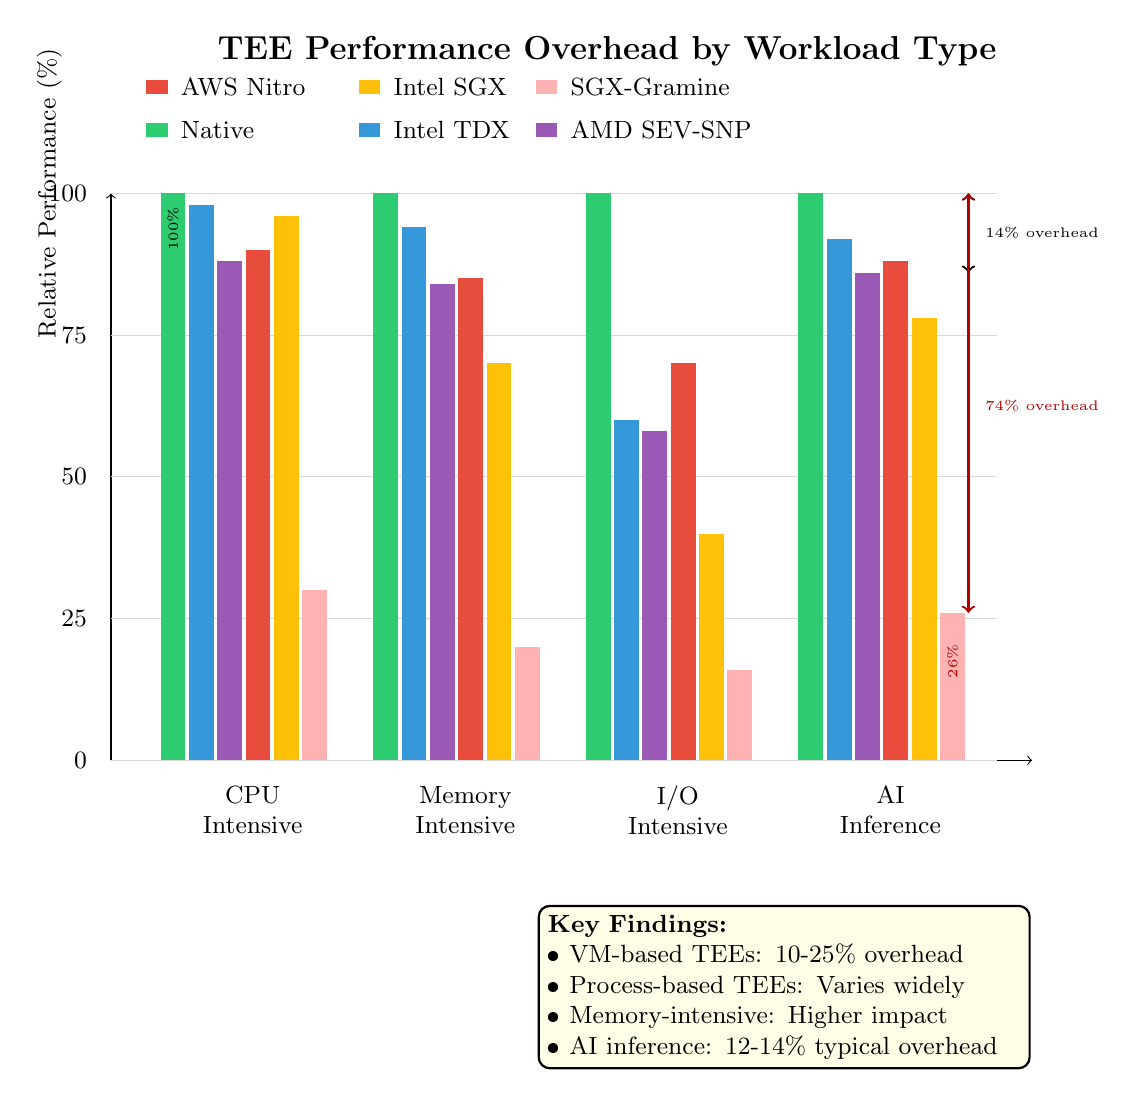
\begin{tikzpicture}[scale=0.9]
    % Define colors
    \definecolor{nativecolor}{RGB}{46, 204, 113}
    \definecolor{tdxcolor}{RGB}{52, 152, 219}
    \definecolor{sevcolor}{RGB}{155, 89, 182}
    \definecolor{nitrocolor}{RGB}{231, 76, 60}
    \definecolor{sgxcolor}{RGB}{255, 193, 7}
    
    % Title
    \node[font=\bfseries\large] at (7, 10) {TEE Performance Overhead by Workload Type};
    
    % Axes
    \draw[->] (0, 0) -- (0, 8) node[anchor=south, rotate=90, yshift=0.5cm, font=\small] {Relative Performance (\%)};
    \draw[->] (0, 0) -- (13, 0);
    
    % Y-axis labels
    \foreach \y/\label in {0/0, 2/25, 4/50, 6/75, 8/100} {
        \draw[gray!30, thin] (0, \y) -- (12.5, \y);
        \node[anchor=east, font=\small] at (-0.2, \y) {\label};
    }
    
    % Workload categories
    \node[font=\small, text width=2cm, align=center] at (2, -0.7) {CPU\\Intensive};
    \node[font=\small, text width=2cm, align=center] at (5, -0.7) {Memory\\Intensive};
    \node[font=\small, text width=2cm, align=center] at (8, -0.7) {I/O\\Intensive};
    \node[font=\small, text width=2cm, align=center] at (11, -0.7) {AI\\Inference};
    
    % Bar width
    \def\barwidth{0.35}
    
    % CPU Intensive workload
    \fill[nativecolor] (0.7, 0) rectangle (0.7+\barwidth, 8); % Native = 100%
    \fill[tdxcolor] (1.1, 0) rectangle (1.1+\barwidth, 7.84); % TDX = 98%
    \fill[sevcolor] (1.5, 0) rectangle (1.5+\barwidth, 7.04); % SEV = 88%
    \fill[nitrocolor] (1.9, 0) rectangle (1.9+\barwidth, 7.2); % Nitro = 90%
    \fill[sgxcolor] (2.3, 0) rectangle (2.3+\barwidth, 7.68); % SGX = 96%
    \fill[red!30] (2.7, 0) rectangle (2.7+\barwidth, 2.4); % SGX-Gramine = 30%
    
    % Memory Intensive workload
    \fill[nativecolor] (3.7, 0) rectangle (3.7+\barwidth, 8);
    \fill[tdxcolor] (4.1, 0) rectangle (4.1+\barwidth, 7.52); % 94%
    \fill[sevcolor] (4.5, 0) rectangle (4.5+\barwidth, 6.72); % 84%
    \fill[nitrocolor] (4.9, 0) rectangle (4.9+\barwidth, 6.8); % 85%
    \fill[sgxcolor] (5.3, 0) rectangle (5.3+\barwidth, 5.6); % 70%
    \fill[red!30] (5.7, 0) rectangle (5.7+\barwidth, 1.6); % 20%
    
    % I/O Intensive workload
    \fill[nativecolor] (6.7, 0) rectangle (6.7+\barwidth, 8);
    \fill[tdxcolor] (7.1, 0) rectangle (7.1+\barwidth, 4.8); % 60%
    \fill[sevcolor] (7.5, 0) rectangle (7.5+\barwidth, 4.64); % 58%
    \fill[nitrocolor] (7.9, 0) rectangle (7.9+\barwidth, 5.6); % 70%
    \fill[sgxcolor] (8.3, 0) rectangle (8.3+\barwidth, 3.2); % 40%
    \fill[red!30] (8.7, 0) rectangle (8.7+\barwidth, 1.28); % 16%
    
    % AI Inference workload
    \fill[nativecolor] (9.7, 0) rectangle (9.7+\barwidth, 8);
    \fill[tdxcolor] (10.1, 0) rectangle (10.1+\barwidth, 7.36); % 92%
    \fill[sevcolor] (10.5, 0) rectangle (10.5+\barwidth, 6.88); % 86%
    \fill[nitrocolor] (10.9, 0) rectangle (10.9+\barwidth, 7.04); % 88%
    \fill[sgxcolor] (11.3, 0) rectangle (11.3+\barwidth, 6.24); % 78%
    \fill[red!30] (11.7, 0) rectangle (11.7+\barwidth, 2.08); % 26%
    
    % Performance labels on selected bars
    \node[font=\tiny, rotate=90] at (0.7+\barwidth/2, 7.5) {100\%};
    \node[font=\tiny, rotate=90, tdxcolor] at (10.1+\barwidth/2, 6.8) {92\%};
    \node[font=\tiny, rotate=90, sevcolor] at (10.5+\barwidth/2, 6.3) {86\%};
    \node[font=\tiny, rotate=90, nitrocolor] at (10.9+\barwidth/2, 6.4) {88\%};
    \node[font=\tiny, rotate=90, sgxcolor] at (11.3+\barwidth/2, 5.6) {78\%};
    \node[font=\tiny, rotate=90, red!70!black] at (11.7+\barwidth/2, 1.4) {26\%};
    
    % Overhead annotations (moved to right side)
    \draw[<->, thick] (12.1, 6.88) -- (12.1, 8);
    \node[font=\tiny, anchor=west] at (12.2, 7.44) {14\% overhead};
    
    \draw[<->, thick, red!70!black] (12.1, 2.08) -- (12.1, 8);
    \node[font=\tiny, anchor=west, red!70!black] at (12.2, 5) {74\% overhead};
    
    % Legend - moved above the plot with better spacing
    \fill[nativecolor] (0.5, 8.8) rectangle (0.8, 9.0);
    \node[anchor=west, font=\small] at (0.85, 8.9) {Native};
    
    \fill[tdxcolor] (3.5, 8.8) rectangle (3.8, 9.0);
    \node[anchor=west, font=\small] at (3.85, 8.9) {Intel TDX};
    
    \fill[sevcolor] (6.0, 8.8) rectangle (6.3, 9.0);
    \node[anchor=west, font=\small] at (6.35, 8.9) {AMD SEV-SNP};
    
    \fill[nitrocolor] (0.5, 9.4) rectangle (0.8, 9.6);
    \node[anchor=west, font=\small] at (0.85, 9.5) {AWS Nitro};
    
    \fill[sgxcolor] (3.5, 9.4) rectangle (3.8, 9.6);
    \node[anchor=west, font=\small] at (3.85, 9.5) {Intel SGX};
    
    \fill[red!30] (6.0, 9.4) rectangle (6.3, 9.6);
    \node[anchor=west, font=\small] at (6.35, 9.5) {SGX-Gramine};
    
    % Key finding box - moved further down, outside plot area
    \node[draw, thick, rounded corners, fill=yellow!10, text width=6cm, align=left, font=\small] at (9.5, -3.2) {
        \textbf{Key Findings:}\\
        • VM-based TEEs: 10-25\% overhead\\
        • Process-based TEEs: Varies widely\\
        • Memory-intensive: Higher impact\\
        • AI inference: 12-14\% typical overhead
    };
    
\end{tikzpicture}
\caption{Performance comparison across TEE implementations for different workload characteristics. VM-based TEEs (TDX, SEV-SNP, Nitro) demonstrate consistent 10-25\% overhead for AI inference, while process-based SGX shows severe degradation for memory-intensive workloads when exceeding EPC capacity.}
\label{fig:performance_overhead}
\end{figure}

For CPU-intensive workloads including TensorFlow and PyTorch inference operations, the research found that virtual machine-based TEEs impose modest overhead compared to native execution. Intel TDX demonstrated excellent performance approaching or occasionally exceeding native execution due to optimization of memory encryption operations. AMD SEV-SNP showed 10 to 15 percent overhead primarily attributable to the computational cost of memory encryption and decryption on every memory access \cite{tee_evolution}. AWS Nitro Enclaves falls within a similar range based on its VM-based architecture, though specific benchmarks in the published research did not include Nitro measurements. Process-based SGX implementations using the Gramine runtime approached native performance for CPU-bound operations where the small Enclave Page Cache did not constrain execution \cite{gramine}.

These CPU overhead measurements indicate that the processor execution of model inference code itself does not suffer dramatic slowdowns within TEEs. The mathematical operations underlying neural network inference including matrix multiplications, activation functions, and normalization computations execute at near-native speeds. The overhead stems primarily from memory encryption and context switching between secure and non-secure execution rather than from the inference computations themselves. For AI workloads where computation dominates memory access patterns, the overhead remains acceptably low at 10 to 25 percent slower than unprotected execution.

Memory-intensive workloads demonstrate more pronounced performance differences between TEE implementations. The research measured Redis and Vault performance, representing applications with high memory access rates relative to computation. Intel TDX achieved highest throughput with latency comparable to native execution, demonstrating the maturity of its memory encryption implementation \cite{tee_evolution}. AMD SEV-SNP showed 15 to 20 percent overhead accounting for differences in processor performance characteristics. Gramine-SGX exhibited worst performance with severe degradation due to the limited Enclave Page Cache forcing frequent swapping between encrypted and unencrypted memory regions \cite{gramine}. The Occlum SGX runtime similarly struggled with memory-intensive loads, confirming that process-based TEEs fundamentally cannot compete with VM-based alternatives for applications requiring substantial memory working sets.

For artificial intelligence inference workloads, the memory access patterns depend on model architecture and batch size. Transformer-based language models exhibit memory-intensive characteristics due to attention mechanisms that access large portions of model state for each token processed. Convolutional neural networks for computer vision applications show more favorable cache locality with repeated access to small kernel weights. The memory intensity of AI workloads positions them closer to the memory-intensive benchmark category than pure CPU-intensive computation, suggesting that the 15 to 25 percent overhead range represents realistic expectations for large language model inference in TEEs.

Input-output-intensive workloads including NGINX web server and Node.js application server revealed substantial overhead from TEE isolation mechanisms. Intel TDX and AMD SEV-SNP both demonstrated approximately 40 percent overhead compared to native execution \cite{tee_evolution}. The Gramine-SGX and Occlum-SGX process-based implementations could not sustain high concurrent request rates, experiencing failures under load. The input-output overhead stems from the additional security checks, context switches, and encryption operations required for each I/O operation crossing security boundaries. For AI inference services exposed through network APIs, this I/O overhead compounds with the computational overhead of inference itself.

The vsock communication mechanism used by AWS Nitro Enclaves provides favorable performance characteristics compared to general network I/O. Measurements indicate round-trip latency between 100 and 500 microseconds for vsock communication with bandwidth capabilities reaching 10 to 20 gigabits per second \cite{nitro_security}. These characteristics prove sufficient for typical inference request patterns where the computation time for model inference measured in milliseconds or seconds far exceeds the communication overhead. The lack of external networking eliminates network protocol processing overhead that contributes to the I/O overhead observed in benchmarks of network-connected TEE applications.

\subsection{Optimization Strategies for Production Deployment}

Optimizing TEE-based AI systems for production deployment requires addressing multiple dimensions including model size reduction, batching strategies, caching approaches, and infrastructure configuration. These optimization techniques can substantially improve performance and reduce costs while maintaining acceptable accuracy and security properties. The specific optimizations appropriate for a deployment depend on the workload characteristics, latency requirements, and cost constraints of the application.

Model quantization represents the most impactful optimization for reducing memory requirements and improving inference speed. The process of quantization converts model weights and potentially activations from higher-precision floating point representations to lower-precision formats including 8-bit integers \cite{quantization_survey}. Post-training quantization techniques can be applied to pre-trained models without requiring retraining, making them accessible for deploying existing models. Quantization-aware training integrates quantization simulation during the training process, enabling models to adapt to reduced precision and maintain higher accuracy. The accuracy impact of quantization varies by model architecture and task, with well-designed quantization achieving less than 1 to 2 percent accuracy degradation on many benchmarks.

The memory reduction from quantization directly translates to cost savings through the ability to use smaller instance types. A model requiring 52 gigabytes in 16-bit floating point format can be quantized to 8-bit integers requiring only 26 gigabytes, potentially enabling deployment on an instance type half the size at corresponding cost reduction. The reduced memory bandwidth requirements from quantization also improve inference throughput by reducing memory transfer time. The computational operations on quantized values can leverage specialized processor instructions for integer arithmetic, further accelerating inference compared to floating point computation \cite{quantization_survey}.

Knowledge distillation provides an alternative approach to model size reduction through training smaller models that approximate the behavior of larger teacher models \cite{knowledge_distillation}. The distilled student model learns to mimic the teacher's outputs across a training dataset, often achieving 80 to 90 percent of the teacher's accuracy with substantially fewer parameters. A 7 billion parameter model might be distilled to 1 billion parameters, reducing memory requirements by a factor of seven while maintaining useful predictive performance. Distillation enables deployment scenarios where even quantized full-size models exceed memory capacity, though the accuracy trade-offs require careful evaluation for specific applications.

Model pruning techniques remove redundant parameters that contribute minimally to model accuracy, creating sparse models with reduced memory footprint \cite{model_pruning}. Structured pruning removes entire neurons, attention heads, or layers from the model architecture, maintaining dense computation patterns that leverage standard hardware efficiently. Unstructured pruning removes individual weights based on magnitude or importance criteria, achieving higher sparsity but requiring specialized sparse computation kernels for performance benefits. Pruning can reduce model size by 30 to 50 percent with minimal accuracy loss, combining effectively with quantization for compound compression. The irregular memory access patterns of sparse models may interact unfavorably with TEE memory encryption, requiring empirical evaluation of performance impact.

Batch processing of inference requests amortizes fixed overhead costs across multiple predictions, improving overall throughput at the cost of increased latency for individual requests \cite{batch_processing}. The overhead from memory encryption, context switching, and security checks occurs once per batch rather than per request, reducing the proportional impact as batch size increases. Batching also improves hardware utilization by enabling more efficient use of processor parallelism through vectorized operations across batch elements. The optimal batch size balances between latency requirements that favor small batches and throughput optimization that favors large batches. Typical production deployments use batch sizes ranging from 4 to 32 depending on latency targets and request arrival patterns.

Caching strategies reduce redundant computation by storing and reusing inference results for repeated or similar queries. Model weights can be cached in enclave memory across multiple inference requests, avoiding repeated decryption from encrypted storage. Intermediate layer activations can be cached for requests sharing common prefixes in sequential processing tasks, enabling faster completion of related queries. The AWS Key Management Service integration benefits from caching decrypted data keys to avoid repeated KMS API calls for the same encryption key \cite{kms_integration}. Caching must be implemented carefully to avoid information leakage through cache side channels or timing variations that could reveal which queries share cached results.

Pre-warming enclaves during deployment reduces the latency experienced by initial requests after enclave startup. The pre-warming process loads model weights, performs compilation or optimization of inference code, and potentially executes sample inference operations to populate caches and optimize execution paths. This initialization cost occurs once during enclave launch rather than on the first user request, improving user-perceived performance. The trade-off involves consuming resources during pre-warming that could otherwise be used for serving requests, requiring capacity planning to balance initialization overhead against request serving capacity.

Infrastructure configuration optimization addresses system-level factors affecting performance. Selecting instance types with appropriate CPU, memory, and network characteristics for the workload maximizes resource efficiency. Memory-optimized instances provide cost-effective deployment for large models with high memory requirements relative to CPU usage. Compute-optimized instances suit scenarios where inference computation dominates memory access. Placement of parent instances in regions with low network latency to clients reduces end-to-end response time. The allocation of vCPUs and memory to enclaves relative to parent instances affects both performance and security, with isolated dedicated resources improving performance predictability at the cost of reduced flexibility.

\subsection{Cost-Benefit Analysis for TEE Deployment}

Evaluating the economic viability of TEE-based AI deployments requires analyzing both the additional costs imposed by security mechanisms and the benefits derived from verifiable computation, model protection, and regulatory compliance. The cost structure for TEE deployments differs from conventional deployments primarily through increased infrastructure requirements and operational complexity, while benefits manifest through expanded addressable markets, reduced trust requirements, and competitive differentiation.

The compute cost differential for AWS Nitro Enclaves is minimal in direct terms because AWS does not charge additional fees specifically for enclave capabilities beyond standard EC2 instance pricing \cite{nitro_security}. However, the performance overhead of 10 to 25 percent means that serving equivalent workload throughput requires proportionally more compute capacity compared to native execution. An application that could serve 1000 requests per second on bare instances might require instances capable of 1200 to 1250 requests per second to maintain throughput when deployed in enclaves. This capacity increase translates to 20 to 25 percent higher compute costs purely from performance overhead.

The memory overhead from requiring larger instance types to accommodate model sizes and activation memory further increases costs. A model that would fit in a 16 gigabyte instance without TEE protection might require a 32 or 64 gigabyte instance when accounting for enclave memory allocation, EIF decompression, and safety margins for memory fragmentation. Memory-optimized instances command premium pricing compared to general-purpose instances with equivalent CPU capacity, adding 30 to 50 percent to infrastructure costs for memory-intensive AI workloads. The combined impact of performance overhead and memory requirements suggests that TEE deployment increases direct compute costs by approximately 40 to 60 percent compared to equivalent unprotected deployments.

Operational costs increase due to the additional complexity of managing encrypted models, certificate rotation, attestation verification, and blockchain integration. Development costs rise through requirements for specialized expertise in TEE programming, cryptographic protocol implementation, and security analysis. The need for security audits of enclave code and attestation policies adds periodic expenses throughout the application lifecycle. Monitoring and incident response processes must adapt to the unique characteristics of enclave environments where traditional debugging and introspection tools cannot access protected memory. These operational and development cost increases are difficult to quantify precisely but represent substantial multipliers on initial implementation effort and ongoing maintenance burden.

The benefits of TEE deployment justify these increased costs for applications where verifiable computation, model protection, or regulatory compliance create significant value. Decentralized AI networks fundamentally require verifiable computation to establish trust among mutually distrusting participants, making the cost of TEE deployment a necessary condition for market existence rather than an optional enhancement \cite{confidential_computing}. Model providers can monetize valuable models in decentralized markets only if they have confidence that model weights will not be stolen, with TEE-based protection enabling business models otherwise foreclosed by intellectual property concerns. The expansion of addressable market through enabling decentralized participation may generate revenue increases that dwarf the incremental infrastructure costs.

Regulatory compliance requirements in healthcare, finance, and other regulated industries often mandate confidential computing approaches for processing sensitive data \cite{gdpr_compliance, hipaa_security}. The cost of TEE deployment becomes a compliance expense necessary for legal operation rather than an optional security enhancement. Organizations may find that TEE-based approaches enable processing of data that would otherwise be prohibited, creating new business opportunities with associated revenue potential. The cost of non-compliance through data breaches, regulatory fines, or legal liability far exceeds the incremental cost of TEE deployment, making confidential computing economically rational from a risk management perspective.

Competitive differentiation through verifiable AI can command premium pricing from customers who value transparency and trust. Organizations may be willing to pay substantially more for AI services with cryptographic proof of model identity and correct execution compared to opaque alternatives. The ability to market services as independently verifiable and cryptographically protected from provider manipulation represents significant brand value in markets where trust is paramount. This pricing power can offset infrastructure costs through revenue increases rather than cost reduction.

Insurance and liability considerations favor TEE deployment by reducing exposure to data breach costs and regulatory penalties. Organizations processing sensitive data within TEEs can negotiate more favorable cyber insurance premiums by demonstrating strong technical controls. The cryptographic audit trail provided by attestation mechanisms facilitates incident response and forensics when security events occur. These risk management benefits have quantifiable financial value through reduced expected costs of security incidents weighted by probability of occurrence.

\subsection{Scalability Considerations and Limitations}

The scalability characteristics of TEE-based AI systems determine their suitability for deployment at various scales from individual experimental deployments to large production networks serving millions of requests. Understanding scalability limitations and mitigation strategies informs architecture decisions and capacity planning for growing systems. The scalability challenges differ between vertical scaling of individual nodes and horizontal scaling across multiple nodes in distributed deployments.

Vertical scaling through deployment on larger instance types with more CPU cores and memory capacity faces diminishing returns beyond certain thresholds. AWS Nitro Enclaves supports allocation of multiple vCPUs to enclaves, enabling parallelism within model inference for operations that can be decomposed across processors. However, the maximum allocation is constrained by the parent instance size, limiting vertical scaling to the largest available instance types. Memory bandwidth becomes a bottleneck for very large models where the rate of weight access during inference saturates available bandwidth regardless of CPU capacity \cite{memory_bandwidth}. The memory encryption operations in TEEs consume additional bandwidth, potentially exacerbating bandwidth constraints compared to native execution.

Horizontal scaling through deploying multiple enclave instances across a cluster of machines provides more flexible capacity scaling. Load balancers distribute requests across multiple enclave endpoints, enabling linear scaling of throughput with node count. Each enclave instance operates independently with its own model copy and attestation identity, simplifying the architecture compared to distributed inference approaches. The challenge in horizontal scaling centers on maintaining consistent attestation verification across a growing fleet of enclaves, requiring efficient mechanisms for nodes to prove their trustworthiness continuously.

The certificate rotation requirement where enclave attestation certificates expire after three hours creates operational challenges for large-scale deployments \cite{nitro_security}. Each enclave must periodically regenerate attestation documents and update any external registries or verifiers with fresh attestation evidence. Coordinating certificate rotation across thousands of enclaves requires robust automation to prevent service disruptions from expired attestations. The blast radius of automation failures could render entire fleets unable to prove their authenticity simultaneously if rotation logic fails. Best practices involve staggered rotation schedules and graceful degradation where enclaves approaching expiration time receive reduced load while renewed enclaves handle increasing traffic.

The blockchain interaction overhead from on-chain attestation verification poses scalability challenges due to transaction throughput limits and gas costs. Public blockchain networks process limited transactions per second, creating bottlenecks when large numbers of enclaves attempt to register or refresh attestations simultaneously \cite{blockchain_consensus}. The gas costs for on-chain verification scale linearly with the number of enclaves, potentially becoming prohibitively expensive for large fleets. Scalability requires off-chain verification patterns where specialized nodes verify attestations and commit only compact proofs to blockchain storage, enabling one on-chain transaction to represent verification of many enclaves.

The coordination overhead for distributed inference across multiple enclaves becomes significant for architectures that split individual requests across nodes. Techniques such as pipeline parallelism that partition model layers across enclaves or tensor parallelism that split layer computations across multiple processors require tight synchronization and data transfer \cite{model_serving}. The vsock communication model where enclaves cannot directly communicate creates challenges for distributed inference patterns, requiring all coordination to flow through parent instances or external systems. The added latency and complexity of multi-enclave inference may outweigh the benefits except for extremely large models that cannot fit within single enclave memory.

The monitoring and observability scalability challenges arise from restrictions on data exposure from secure enclaves. Traditional monitoring approaches that instrument code to emit detailed telemetry cannot be applied directly within enclaves without risking information leakage. Aggregating monitoring data from large enclave fleets requires careful filtering to remove sensitive information while retaining operationally useful signals. The inability to attach debuggers or profilers to running enclaves complicates performance troubleshooting at scale, necessitating alternative approaches based on structured logging through secure channels and statistical analysis of aggregate behavior \cite{monitoring_systems}.

The state management complexity increases with scale as enclaves cannot maintain persistent state locally but must externalize any data requiring durability. Large deployments require external state management systems that handle encrypted state from thousands of enclaves, implement efficient key management at scale, and provide low-latency access to state data. The proliferation of encryption keys across large enclave fleets creates key management challenges including secure distribution, rotation, and revocation. The scalability of external systems that support enclave deployments such as key management services and certificate authorities becomes critical to overall system scalability.

Despite these challenges, practical deployments have demonstrated that TEE-based AI systems can scale to meaningful production workloads. The fundamental architecture of independent enclave instances handling requests without requiring coordination between instances enables straightforward horizontal scaling for stateless inference workloads. The performance overhead remains acceptable for applications where security and verifiability justify the cost. The operational complexity can be managed through appropriate automation and monitoring infrastructure. Organizations deploying at scale should invest in robust orchestration systems, implement comprehensive observability, and design for graceful degradation when components fail. The scalability of TEE-based AI systems is limited more by operational maturity and cost considerations than by fundamental technical constraints of the TEE technology itself.